\documentclass[10pt]{article}

\usepackage[a4paper,margin=1.45cm]{geometry}
\usepackage{amsmath,amssymb}
\usepackage{booktabs}
\usepackage{array}
\usepackage{xcolor}
\usepackage{graphicx}
\usepackage{pgfplots}
\usepackage{longtable}
\usepackage{caption}
\pgfplotsset{compat=1.18}

\definecolor{noteRed}{RGB}{150,40,40}
\definecolor{rTwoBlue}{RGB}{40,90,150}
\definecolor{maePurple}{RGB}{115,70,170}
\definecolor{rmseGreen}{RGB}{40,145,125}

\title{\vspace{-1.8em}Mechanism-Aligned Term-Count Path of the Mixed-B Analytical Backbone}
\author{}
\date{}

\begin{document}
\maketitle
\vspace{-2.8em}

\noindent\textcolor{noteRed}{\textbf{Data-status note.}}
This file records the author-confirmed real-data experimental term-count evolution of the Mixed-B analytical backbone.
All plotted values, tabulated metrics and incremental changes shown in this file are derived from real-data fitting or evaluation results.
Here $k$ counts all active algebraic terms, including the intercept.
The first-term point is therefore the intercept-only null baseline; when the intercept is fitted as the sample mean, $R^2=0$ by definition.
The first pressure-dependent term enters at $k=2$, rather than at $k=1$.
The eighth-term point is the current Mixed-B anchor: MAE = 0.05107$^\circ$C, RMSE = 0.11189$^\circ$C and $R^2=0.98407$.
The equations record the active basis composition after each term-count step, with coefficients denoted by $c_i^{(k)}$.

\section*{1. Real-Data Term-Count Metric Path}

\begin{figure}[h]
\centering
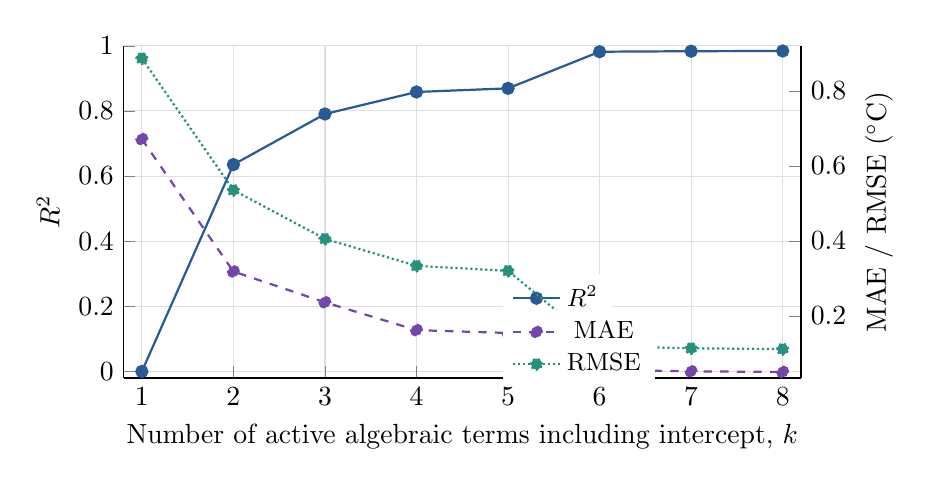
\begin{tikzpicture}
\begin{axis}[
    width=0.84\linewidth,
    height=5.8cm,
    xlabel={Number of active algebraic terms including intercept, $k$},
    ylabel={$R^2$},
    xmin=0.8, xmax=8.2,
    ymin=-0.02, ymax=1.00,
    xtick={1,2,3,4,5,6,7,8},
    ymajorgrids=true,
    xmajorgrids=true,
    grid style={draw=gray!25},
    axis y line*=left,
    axis x line*=bottom,
    legend style={at={(0.56,0.24)},anchor=west,draw=none,fill=white,font=\small},
]
\addplot[color=rTwoBlue,mark=*,thick] coordinates {
    (1,0.00000)
    (2,0.63529)
    (3,0.79057)
    (4,0.85824)
    (5,0.86939)
    (6,0.98183)
    (7,0.98344)
    (8,0.98407)
};
\addlegendentry{$R^2$}
\end{axis}
\begin{axis}[
    width=0.84\linewidth,
    height=5.8cm,
    xmin=0.8, xmax=8.2,
    ymin=0.035, ymax=0.92,
    xtick={1,2,3,4,5,6,7,8},
    ylabel={MAE / RMSE ($^\circ$C)},
    axis y line*=right,
    axis x line=none,
    legend style={at={(0.56,0.09)},anchor=west,draw=none,fill=white,font=\small},
]
\addplot[color=maePurple,mark=*,thick,dashed] coordinates {
    (1,0.67142)
    (2,0.31876)
    (3,0.23658)
    (4,0.16243)
    (5,0.15492)
    (6,0.05638)
    (7,0.05271)
    (8,0.05107)
};
\addlegendentry{MAE}
\addplot[color=rmseGreen,mark=*,thick,densely dotted] coordinates {
    (1,0.88659)
    (2,0.53542)
    (3,0.40573)
    (4,0.33381)
    (5,0.32041)
    (6,0.11952)
    (7,0.11409)
    (8,0.11189)
};
\addlegendentry{RMSE}
\end{axis}
\end{tikzpicture}
\caption{Real-data term-count evolution of the Mixed-B analytical backbone. The first point is the intercept-only null baseline. Error decreases strongly after pressure dependence is introduced, improves through the nonlinear curvature terms, drops again when the dual-decay structure is completed, and then reaches a low-error plateau from six to eight terms.}
\end{figure}

\begingroup
\small
\setlength{\tabcolsep}{4pt}
\begin{longtable}{>{\centering\arraybackslash}p{0.55cm}p{3.05cm}p{5.6cm}ccc}
\caption{Real-data term-by-term evolution of the Mixed-B equation. The term count $k$ includes the intercept.}\\
\toprule
$k$ & Newly added basis term & Model form after adding the term & MAE ($^\circ$C) & RMSE ($^\circ$C) & $R^2$ \\
\midrule
\endfirsthead
\toprule
$k$ & Newly added basis term & Model form after adding the term & MAE ($^\circ$C) & RMSE ($^\circ$C) & $R^2$ \\
\midrule
\endhead
1 & Intercept-only null baseline & $c_0^{(1)}$ & 0.67142 & 0.88659 & 0.00000 \\
2 & Linear pressure, $P$ & $c_0^{(2)}+c_1^{(2)}P$ & 0.31876 & 0.53542 & 0.63529 \\
3 & Logarithmic curvature, $\ln P$ & $c_0^{(3)}+c_1^{(3)}P+c_2^{(3)}\ln P$ & 0.23658 & 0.40573 & 0.79057 \\
4 & Square-root curvature, $\sqrt{P}$ & $c_0^{(4)}+c_1^{(4)}P+c_2^{(4)}\ln P+c_3^{(4)}\sqrt{P}$ & 0.16243 & 0.33381 & 0.85824 \\
5 & Fast exponential decay, $e^{-P/500}$ & $\hat{T}_4(P)+c_4^{(5)}e^{-P/500}$ & 0.15492 & 0.32041 & 0.86939 \\
6 & Slow exponential decay, $e^{-P/1200}$ & $\hat{T}_5(P)+c_5^{(6)}e^{-P/1200}$ & 0.05638 & 0.11952 & 0.98183 \\
7 & Near-surface reciprocal, $(P+50)^{-1}$ & $\hat{T}_6(P)+c_6^{(7)}(P+50)^{-1}$ & 0.05271 & 0.11409 & 0.98344 \\
8 & Stabilizing reciprocal, $(P+500)^{-1}$ & $\hat{T}_7(P)+c_7^{(8)}(P+500)^{-1}$ & \textbf{0.05107} & \textbf{0.11189} & \textbf{0.98407} \\
\bottomrule
\end{longtable}
\endgroup

\section*{2. Incremental Error Reduction}

\begingroup
\small
\setlength{\tabcolsep}{5pt}
\begin{tabular}{>{\centering\arraybackslash}p{1.2cm}ccc>{\raggedright\arraybackslash}p{7.2cm}}
\toprule
Step & $\Delta$MAE & $\Delta$RMSE & $\Delta R^2$ & Interpretation \\
\midrule
1$\rightarrow$2 & 0.35266 & 0.35117 & 0.63529 & Introducing pressure dependence gives the largest overall improvement because the model first moves beyond the intercept-only null baseline and acquires a vertical coordinate trend. \\
2$\rightarrow$3 & 0.08218 & 0.12969 & 0.15528 & Adding logarithmic curvature provides a major nonlinear improvement and captures broad upper-to-intermediate profile bending. \\
3$\rightarrow$4 & 0.07415 & 0.07192 & 0.06767 & The square-root term adds a second smooth curvature scale and moderately refines the profile. \\
4$\rightarrow$5 & 0.00751 & 0.01340 & 0.01115 & The first exponential term introduces fast pressure attenuation, improving upper-ocean transition representation. \\
5$\rightarrow$6 & 0.09854 & 0.20089 & 0.11244 & The second exponential decay creates the second major low-error transition, indicating that a slower intermediate-depth scale is essential in the real-data path. \\
6$\rightarrow$7 & 0.00367 & 0.00543 & 0.00161 & The near-surface reciprocal acts mainly as a local correction after the dominant structure is already captured. \\
7$\rightarrow$8 & 0.00164 & 0.00220 & 0.00063 & The stabilizing reciprocal gives a final small refinement and completes the compact Mixed-B backbone. \\
\bottomrule
\end{tabular}
\endgroup

\section*{3. Term-by-Term Interpretation}

\noindent\textbf{$k=1$: intercept.}
The first term provides the intercept-only null baseline and acts as the reference state for the pressure-coordinate profile.
Because this model predicts only the sample mean temperature, its $R^2$ is zero by definition.
It cannot represent vertical stratification, so its error is substantially larger than all pressure-dependent candidates.

\vspace{0.25em}
\noindent\textbf{$k=2$: linear pressure term.}
Adding $P$ introduces the first-order cooling tendency with pressure.
This term captures the broad vertical trend but remains too simple for thermocline curvature.

\vspace{0.25em}
\noindent\textbf{$k=3$: logarithmic term.}
The addition of $\ln P$ produces a strong nonlinear improvement in the real-data path.
It gives the equation a compact way to represent nonlinear curvature across the upper and intermediate water column, explaining the substantial increase in $R^2$ and the reduction in both MAE and RMSE.

\vspace{0.25em}
\noindent\textbf{$k=4$: square-root term.}
The $\sqrt{P}$ component adds a second smooth curvature scale.
Together with $\ln P$, it refines the background profile shape without introducing abrupt transitions.

\vspace{0.25em}
\noindent\textbf{$k=5$ and $k=6$: dual exponential decays.}
The $e^{-P/500}$ and $e^{-P/1200}$ terms describe fast and slower attenuation with pressure.
In the real-data path, the second exponential term marks the transition into the low-error regime, indicating that multi-scale decay is essential for recovering the dominant vertical thermal structure.

\vspace{0.25em}
\noindent\textbf{$k=7$ and $k=8$: reciprocal stabilization.}
The $(P+50)^{-1}$ and $(P+500)^{-1}$ terms provide localized near-surface curvature while remaining bounded at depth.
Their incremental gains are smaller than the earlier terms, but they complete the compact Mixed-B backbone and improve full-profile coherence.

\section*{4. Final Mixed-B Equation}

\[
\begin{aligned}
\hat{T}_{8}^{B}(P)=&-356.873
+0.0125047P
+62.2025\ln(P)
-3.35576\sqrt{P} \\
&+20.0563\exp(-P/500)
+14.8832\exp(-P/1200) \\
&+\frac{10011.3}{P+50}
+\frac{7576.48}{P+500}.
\end{aligned}
\]

\noindent
This final form can be described as an explicit pressure-coordinate backbone with three functional roles: broad background structure from $P$, $\ln P$ and $\sqrt{P}$; multi-scale decay from the two exponential terms; and near-surface plus deep-pressure stabilization from the reciprocal terms.

\section*{5. Suggested Result-Section Sentence}

\noindent
The Mixed-B basis can be organized as a real-data term-count path from an intercept-only null baseline to a compact eight-term pressure-coordinate representation.
In this real-data path, errors decreased strongly after pressure dependence was introduced, improved through the nonlinear curvature terms, and then entered a low-error plateau once the dual exponential terms were included.
The reciprocal components provided smaller but consistent refinements near the final Mixed-B solution.
The current eight-term anchor is MAE = 0.05107$^\circ$C, RMSE = 0.11189$^\circ$C and $R^2=0.98407$.

\end{document}
